\chapter{烯烃和炔烃：亲电加成}\label{ch:b1:electrophilic-additions}

将烯烃与橙色的溴水振荡，几秒钟内颜色便消失：
这是检验碳碳双键最古老的方法。其背后是一套
机理。双键的 $\pi$ 电子结合得比
$\sigma$ 电子松散，且暴露在分子平面的上方和下方，
它们进攻\omterm{def:b1:lewis-resonance-vsepr:hypervalent}{缺电子的}试剂，随后生成的\omterm{def:b1:electronic-effects:intermediates}{碳正离子}
再捕获一个\omterm{def:b1:electronic-effects:nucleophile}{亲核试剂}。同样这两步也解释了烯烃与卤化氢、水和卤素的加成，
决定试剂的哪一部分连到哪个碳上，
并确定产物的立体化学。本章将逐一讨论这些内容，
并介绍十九世纪化学家从观察中归纳出的规则，
以及解释该规则的\omterm{def:b1:electronic-effects:intermediates}{碳正离子}。

\begin{recall}
\omterm{def:b1:electronic-effects:intermediates}{碳正离子}及其稳定性和\omterm{def:b1:electronic-effects:curly-arrow}{弯箭头}（见\cref{ch:b1:electronic-effects}）；
哈蒙德假设（\cref{prop:b1:elementary-steps:hammond}）；$Z$/$E$
\omterm{def:b1:stereochemistry-in-depth:isomers}{构型}标记、\cip{R}/\cip{S}、\omterm{def:b1:stereochemistry-in-depth:enantiomers}{内消旋化合物}和\omterm{def:b1:stereochemistry-in-depth:enantiomers}{外消旋混合物}
（见\cref{ch:b1:stereochemistry-in-depth}）。第 1 册（十二年级）只介绍了烯烃的加成反应，
未讲其机理。
\end{recall}

\section{\texorpdfstring{$\pi$}{pi} 键作为亲核试剂}

\begin{definition}[亲电加成]\label{def:b1:electrophilic-additions:electrophilic-addition}
称\emph{亲电加成}\index{亲电加成}为对多重键的一类加成，
其第一步是 $\pi$ 电子进攻\omterm{def:b1:electronic-effects:nucleophile}{亲电试剂} E，
生成\omterm{def:b1:electronic-effects:intermediates}{碳正离子}，
该\omterm{def:b1:electronic-effects:intermediates}{碳正离子}再捕获\omterm{def:b1:electronic-effects:nucleophile}{亲核试剂} Nu，
使 E 和 Nu 分别连到原双键的两个碳上。
\end{definition}

$\pi$ 键是 C=C 中较弱的那个键（见\cref{ch:b1:lewis-resonance-vsepr}），
其电子远离原子核，分布在分子平面的上方和下方：
烯烃是\omterm{def:b1:electronic-effects:nucleophile}{亲核试剂}，能与酸、卤素和其他\omterm{def:b1:electronic-effects:nucleophile}{亲电试剂}反应，
而饱和烷烃与这些试剂不发生作用。

\section{加成卤化氢：马尔科夫尼科夫规则}

\begin{omfigure}
\setchemfig{atom sep=2.1em}
\schemestart
\chemfig{H_3C-[:30]@{c2}CH=[@{pi},,,,]@{c1}CH_2}
\+
\chemfig{@{h}H-[@{hb}]@{br}Br}
\arrow{->}
\chemfig{H_3C-[:30]CH^{+}-[:-30]CH_3}
\+
\chemfig{Br^{-}}
\arrow{->}
\chemfig{H_3C-[:30]CH(-[2]Br)-[:-30]CH_3}
\schemestop
\chemmove{\draw[->, thick, shorten <=2pt, shorten >=2pt](pi) .. controls +(90:7mm) and +(110:7mm) .. (h);
          \draw[->, thick, shorten <=2pt, shorten >=2pt](hb) .. controls +(-90:5mm) and +(-90:5mm) .. (br);}

{\small 溴化氢与丙烯的加成。$\pi$ 电子对夺取质子，
质子连到末端碳上，生成仲\omterm{def:b1:electronic-effects:intermediates}{碳正离子}；
溴离子与之结合，得到 2-溴丙烷。}
\end{omfigure}

\begin{proposition}[马尔科夫尼科夫规则]\label{prop:b1:electrophilic-additions:markovnikov}
在不对称烯烃与 HX 的加成中，氢原子加到
已连有较多氢原子的双键碳上
（\emph{马尔科夫尼科夫规则}\index{马尔科夫尼科夫规则}）。用现代的表述：
\omterm{def:b1:electronic-effects:nucleophile}{亲电试剂}的加成方式应使生成更稳定的\omterm{def:b1:electronic-effects:intermediates}{碳正离子}。
\end{proposition}

\begin{proof}
质子转移是\omterm{def:b1:elementary-steps:rds}{决速步}，为吸热过程，
生成\omterm{def:b1:electronic-effects:intermediates}{碳正离子}。由哈蒙德假设
（\cref{prop:b1:elementary-steps:hammond}）可知，其\omterm{def:b1:elementary-steps:energy-profile}{过渡态}与\omterm{def:b1:electronic-effects:intermediates}{碳正离子}相似，
因此通向更稳定\omterm{def:b1:electronic-effects:intermediates}{碳正离子}的途径\omterm{def:b1:rate-laws:activation-energy}{活化能}较低，
反应也快得多。将质子连到氢较多的碳上，
使正电荷位于烷基较多的碳上，
即更稳定的\omterm{def:b1:electronic-effects:intermediates}{碳正离子}（见\cref{prop:b1:electronic-effects:carbocation-order}）。
\end{proof}

\begin{omfigure}
\begin{tikzpicture}
\begin{axis}[
  width=0.78\linewidth, height=5.0cm, xmin=0, xmax=10, ymin=-45, ymax=125,
  axis x line=bottom, axis y line=left, xlabel={反应坐标},
  ylabel={能量}, xtick=\empty, ytick=\empty, label style={font=\small},
  legend style={font=\scriptsize, draw=none, at={(0.5,-0.30)}, anchor=north}, legend columns=2]
\addplot[omThm, thick, dashed] table[x=x, y=E] {figdata/out/bachelor-1-energy-profiles-primary.dat};
\addplot[omDef, very thick] table[x=x, y=E] {figdata/out/bachelor-1-energy-profiles-secondary.dat};
\legend{经伯碳正离子,经仲碳正离子}
\node[font=\scriptsize, anchor=south] at (axis cs:5,103) {\ce{CH3CH2CH2+}};
\draw[omThm, densely dotted] (axis cs:5,103) -- (axis cs:5,87);
\node[font=\scriptsize, anchor=north] at (axis cs:5,43) {\ce{CH3CH+CH3}};
\node[font=\scriptsize, anchor=north west] at (axis cs:0.1,-3) {丙烯 + HBr};
\end{axis}
\end{tikzpicture}

{\small 溴化氢对丙烯两种可能加成的示意\omterm{def:b1:elementary-steps:energy-profile}{能量曲线}。
较稳定的仲\omterm{def:b1:electronic-effects:intermediates}{碳正离子}能量较低，由哈蒙德假设，
通向它的\omterm{def:b1:elementary-steps:energy-profile}{过渡态}能量也较低：
马尔科夫尼科夫产物生成的速率快得多。}
\end{omfigure}

\begin{definition}[碳正离子重排]\label{def:b1:electrophilic-additions:rearrangement}
称\emph{碳正离子重排}\index{碳正离子重排}为
\omterm{def:b1:electronic-effects:intermediates}{碳正离子}内部氢原子或烷基带着其\omterm{def:b1:lewis-resonance-vsepr:lewis}{成键电子对}，
迁移到相邻的带正电荷的碳上，
生成更稳定的\omterm{def:b1:electronic-effects:intermediates}{碳正离子}（即 1,2-迁移）。
\end{definition}

\begin{example}[甲基迁移]\label{ex:b1:electrophilic-additions:shift}
3,3-二甲基-1-丁烯与氯化氢反应，生成仲\omterm{def:b1:electronic-effects:intermediates}{碳正离子}，
其相邻碳为季碳原子；一个甲基带着其电子对迁移过去，
生成叔\omterm{def:b1:electronic-effects:intermediates}{碳正离子}。主要产物为 2-氯-2,3-二甲基丁烷，
其骨架与烯烃不同；3-氯-2,2-二甲基丁烷
为次要产物。
\end{example}

\begin{omfigure}
\setchemfig{atom sep=2em}
\schemestart
\chemfig{C(-[2]CH_3)(-[6]CH_3)(-[4]H_3C)-CH^{+}-CH_3}
\arrow{->[1,2-迁移]}[,1.5]
\chemfig{C^{+}(-[2]CH_3)(-[4]H_3C)-CH(-[6]CH_3)-CH_3}
\arrow{->[\ce{Cl-}]}
\chemfig{C(-[2]CH_3)(-[6]Cl)(-[4]H_3C)-CH(-[6]CH_3)-CH_3}
\schemestop
\par\vspace{6pt}

{\small 3,3-二甲基丁-2-基正离子的重排：甲基
迁移到带正电的碳上，使仲\omterm{def:b1:electronic-effects:intermediates}{碳正离子}转变为
叔\omterm{def:b1:electronic-effects:intermediates}{碳正离子}，并被氯离子捕获。}
\end{omfigure}

\section{与水加成}

\begin{definition}[烯烃的水合]\label{def:b1:electrophilic-additions:hydration}
烯烃的\emph{水合}\index{水合}是指加入
水，在\omterm{def:b1:predominant-reaction:strong-acid}{强酸}催化下生成醇，是
在\cref{ch:b1:alcohol-activation}中讨论的\omterm{def:b1:alcohol-activation:dehydration}{脱水}的逆过程。
\end{definition}

其机理与 HX 相同，只是以水作\omterm{def:b1:electronic-effects:nucleophile}{亲核试剂}：质子化
（\omterm{prop:b1:electrophilic-additions:markovnikov}{马尔科夫尼科夫规则}），水捕获\omterm{def:b1:electronic-effects:intermediates}{碳正离子}，\omterm{def:b1:electrophilic-additions:hydration}{水合}氢离子
失去一个质子。丙烯生成丙-2-醇，2-甲基丙烯生成
2-甲基丙-2-醇。\omterm{def:b1:electrophilic-additions:hydration}{水合}与\omterm{def:b1:alcohol-activation:dehydration}{脱水}是同一平衡，
\ce{C3H6 + H2O <=> C3H8O}；稀酸水溶液和低温有利于
醇的生成，浓酸、加热以及移除烯烃则有利于
烯烃的生成（见\cref{ch:b1:extent-q-and-k}）。

\section{加卤素：卤正离子与反式加成}

\begin{definition}[卤正离子、反式加成与顺式加成]\label{def:b1:electrophilic-additions:halonium}
在 \ce{Br2} 或 \ce{Cl2} 的加成中，$\pi$ 电子对进攻其中一个
卤原子，同时该卤原子的一对\omterm{def:b1:lewis-resonance-vsepr:lewis}{孤电子对}与第二个碳原子成键，
形成一个三元环状的\emph{卤正离子}\index{卤正离子}，另一卤原子
以卤离子形式离去。若两个新基团位于原双键的
异侧，则称为\emph{反式
加成}\index{反式加成}；位于同侧则为\emph{顺式
加成}\index{顺式加成}。
\end{definition}

\begin{proposition}[卤素加成为反式]\label{prop:b1:electrophilic-additions:anti-addition}
溴对烯烃的加成为\omterm{def:b1:electrophilic-additions:halonium}{反式加成}：\cip{E}-丁-2-烯
得内消旋-2,3-二溴丁烷，\cip{Z}-丁-2-烯则得
\cip{2R,3R}-与\cip{2S,3S}-2,3-二溴丁烷的\omterm{def:b1:stereochemistry-in-depth:enantiomers}{外消旋混合物}。
\end{proposition}

\begin{proof}
溴正离子桥连原双键的一侧；溴负离子
只能从另一侧进攻碳原子，使环开裂，类似于在该碳原子上
发生\omterm{def:b1:stereochemistry-in-depth:isomers}{构型}翻转的 SN2 机理。两个溴原子位于原双键的异侧。
对 \cip{E}-丁-2-烯，进攻任一碳原子所得产物相同，其中
两个\omterm{def:b1:stereochemistry-in-depth:stereocentre}{手性}碳原子互为镜像：\cip{2R,3S}，
为\omterm{def:b1:stereochemistry-in-depth:enantiomers}{内消旋化合物}。对 \cip{Z}-丁-2-烯，一个碳原子进攻得 \cip{2R,3R}，
另一碳原子进攻得 \cip{2S,3S}，两者概率相等，即为\omterm{def:b1:stereochemistry-in-depth:enantiomers}{外消旋混合物}。通过作图的证明见
\cref{exo:b1:electrophilic-additions:10}。
\end{proof}

\begin{omfigure}
\begin{tikzpicture}[font=\small, >={Stealth}]
  % bromonium ion from (E)-but-2-ene
  \coordinate (a) at (0,0); \coordinate (b) at (1.4,0);
  \draw[thick] (a) -- (b);
  \node[circle, fill=white, inner sep=1pt] (br) at (0.7,1.0) {\ce{Br+}};
  \draw[thick] (a) -- (br.south west) (b) -- (br.south east);
  \draw[thick] (a) -- ++(-0.8,0.35) node[left] {H};
  \draw[thick] (a) -- ++(-0.6,-0.6) node[below left] {\ce{CH3}};
  \draw[thick] (b) -- ++(0.8,0.35) node[right] {\ce{CH3}};
  \draw[thick] (b) -- ++(0.6,-0.6) node[below right] {H};
  \node (bm) at (0.7,-1.6) {\ce{Br-}};
  \draw[->, thick, omThm] (bm) to[bend left=25] (0.12,-0.12);
  \node[align=center] at (0.7,-2.4) {从桥接面的对侧进攻};
  \draw[->, thick] (3.3,0) -- (4.4,0);
  \node[align=center] at (6.2,0) {\chemfig{C(-[:150]H_3C)(<[:210]H)(<:[2]Br)-C(<:[:30]H)(-[:-30]CH_3)(<[6]Br)}};
  \node at (6.2,-1.8) {反式产物：内消旋-2,3-二溴丁烷};
\end{tikzpicture}

{\small 由\cip{E}-丁-2-烯形成的溴正离子，及其被
溴负离子从相反一侧开环（\omterm{def:b1:electrophilic-additions:halonium}{反式加成}）。产物具有两个
\omterm{def:b1:stereochemistry-in-depth:isomers}{构型}标记相反的\omterm{def:b1:stereochemistry-in-depth:stereocentre}{手性}碳原子，并在合适\omterm{def:b1:stereochemistry-in-depth:isomers}{构象}中存在内部镜面，
即\omterm{def:b1:stereochemistry-in-depth:enantiomers}{内消旋化合物} \cip{2R,3S}。}
\end{omfigure}

\begin{inthelab}[溴水]
溴是一种密度大、易挥发、剧毒且具腐蚀性的液体。检验
不饱和性时使用稀溴水（或溴\omterm{def:b1:complexation:complex}{配合物}的
商品溶液），在通风橱中操作，每次仅加几滴。
橙色的消失表明发生了加成。在水中，溴正离子
也会被水捕获，同时生成溴代醇，
与二溴化物并存。
\end{inthelab}

\section{炔烃：加成与炔负离子}

炔烃可两次加成 HX 与 \ce{X2}，每步均与烯烃相同（
对 HX 遵循\omterm{prop:b1:electrophilic-additions:markovnikov}{马尔科夫尼科夫规则}）。炔烃的\omterm{def:b1:electrophilic-additions:hydration}{水合}在酸与汞(II)盐催化下进行，
得到的不是预期的不饱和醇，而是酮：烯醇
立即重排为羰基化合物，这一过程在本科二年级分册中研究。

\begin{definition}[端炔、炔负离子]\label{def:b1:electrophilic-additions:acetylide}
三键位于链末端的炔烃 \ce{R-C#C-H} 称为\emph{端炔}\index{端炔}。
\omterm{def:b1:predominant-reaction:strong-acid}{强碱}（氨基钠）可夺去其氢，
生成\emph{炔负离子}\index{炔负离子}
\ce{R-C#C-}，是良好的碳\omterm{def:b1:electronic-effects:nucleophile}{亲核试剂}。
\end{definition}

\begin{proposition}[端炔的酸性]\label{prop:b1:electrophilic-additions:acetylide-acidity}
\omterm{def:b1:electrophilic-additions:acetylide}{端炔}的 C--H 键酸性远强于
烯烃和烷烃的 C--H 键，但仍远弱于水：\omterm{def:b1:electrophilic-additions:acetylide}{炔负离子}
由酰胺离子而非氢氧根生成，并会被水破坏。
\end{proposition}

\begin{proof}
在\omterm{def:b1:electrophilic-additions:acetylide}{炔负离子}中，\omterm{def:b1:lewis-resonance-vsepr:lewis}{孤电子对}占据一个含 50\% \textit{s} 成分的轨道
（\textit{sp} 碳），该轨道比 \textit{sp}$^2$ 或 \textit{sp}$^3$ \omterm{def:b1:electronic-effects:intermediates}{碳负离子}的轨道
更靠近原子核，因而更稳定，其共轭酸也更强。
它仍远比氢氧根碱性强，
故水可使其质子化。
\end{proof}

\omterm{def:b1:electrophilic-additions:acetylide}{炔负离子}可与一级卤代烷发生 SN2 反应（生成新的 C--C 键，
\ce{R-C#C-} + $\mathrm{R'Br}$），或像\omterm{def:b1:organomagnesium:organometallic}{格氏试剂}一样对羰基加成：
这是构建碳骨架的另一种途径。

\begin{method}[预测加成产物]\label{met:b1:electrophilic-additions:predict-addition}
\begin{enumerate}
  \item 确定\omterm{def:b1:electronic-effects:nucleophile}{亲电试剂}（\ce{H+}、\ce{Br2}）
        及随后进攻的\omterm{def:b1:electronic-effects:nucleophile}{亲核试剂}（\ce{X-}、水、卤离子）。
  \item 对于 \ce{H+}：将其加到能生成更稳定的\omterm{def:b1:electronic-effects:intermediates}{碳正离子}的碳上；
        符合马氏规则；检查是否可能发生 1,2-迁移。
  \item 对于 \ce{X2}：形成\omterm{def:b1:electrophilic-additions:halonium}{卤正离子}，并从相对的一面开环
        （\omterm{def:b1:electrophilic-additions:halonium}{反式加成}）；画出两种可能的进攻方式
        并比较产物（内消旋或外消旋）。
  \item 若体系中有水，则还应预期生成醇
        （或卤代醇）。
\end{enumerate}
\end{method}

\begin{history}[弗拉基米尔·马尔科夫尼科夫]
\begin{minipage}[t]{0.2\linewidth}\vspace{0pt}
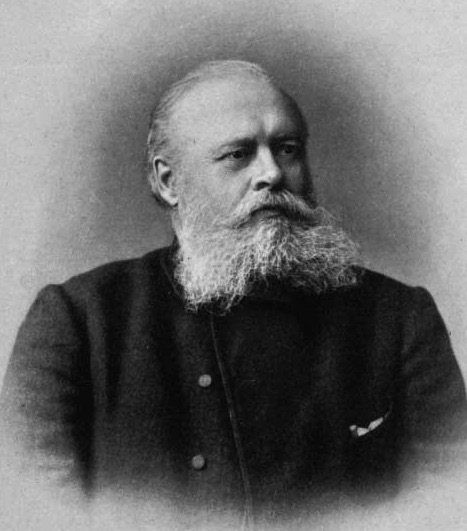
\includegraphics[width=\linewidth]{images/book2/markovnikov.jpg}
\end{minipage}\hfill
\begin{minipage}[t]{0.76\linewidth}\vspace{0pt}
弗拉基米尔·马尔科夫尼科夫于十九世纪提出了他的规则，依据的是他和其他人
观察到的产物，那时\omterm{def:b1:electronic-effects:intermediates}{碳正离子}与\omterm{def:b1:electronic-effects:curly-arrow}{弯箭头}尚未出现：这是一条自然规律，
在能被解释之前已被记录下来。通过\omterm{def:b1:electronic-effects:intermediates}{碳正离子}稳定性给出的现代表述，
清楚地表明机理能为经验规则增添什么：
它指出该规则何时会失效。
（肖像取自 1905 年发表的讣告，公有领域，
维基共享资源。）
\end{minipage}
\end{history}

\section{练习}

\begin{exercise}[$\star$]\label{exo:b1:electrophilic-additions:1}
写出下列反应的主要产物：丙烯 + HCl；2-甲基丙烯 + HBr；
1-甲基环己烯 + HBr；2-丁炔 + 一当量 HCl。
\end{exercise}

\begin{exercise}[$\star$]\label{exo:b1:electrophilic-additions:2}
写出溴分别与乙烯、环己烯和丙烯反应的产物，
并命名。
\end{exercise}

\begin{exercise}[$\star$]\label{exo:b1:electrophilic-additions:3}
各烯烃经酸催化\omterm{def:b1:electrophilic-additions:hydration}{水合}，分别生成哪种醇：
丙烯、2-甲基丙烯、亚甲基环己烷？
\end{exercise}

\begin{exercise}[$\star$]\label{exo:b1:electrophilic-additions:4}
下列化合物中，哪些能与氨基钠反应：丙炔、2-丁炔、
丙烯、乙醇？写出反应式。
\end{exercise}

\begin{exercise}[$\star\star$]\label{exo:b1:electrophilic-additions:5}
用\omterm{def:b1:electronic-effects:curly-arrow}{弯箭头}写出 2-甲基丙烯\omterm{def:b1:electrophilic-additions:hydration}{水合}的完整机理，
并说明为何在热的浓酸中
逆反应更为有利。
\end{exercise}

\begin{exercise}[$\star\star$]\label{exo:b1:electrophilic-additions:6}
用哈蒙德假设解释为何 2-甲基丙烯与 HCl 的反应
远快于丙烯。
\end{exercise}

\begin{exercise}[$\star\star$]\label{exo:b1:electrophilic-additions:7}
溴与环己烯反应。证明产物为
\textit{trans}-1,2-二溴环己烷，并判断其是否具有\omterm{def:b1:stereochemistry-in-depth:stereocentre}{手性}，
以及产物是否具有\omterm{def:b1:stereochemistry-in-depth:optical-activity}{旋光性}。
\end{exercise}

\begin{exercise}[$\star\star$]\label{exo:b1:electrophilic-additions:8}
提出 3-甲基-1-丁烯与 HCl 加成的机理，
使之主要生成 2-氯-2-甲基丁烷。
\end{exercise}

\begin{exercise}[$\star\star$]\label{exo:b1:electrophilic-additions:9}
提出由丙炔与卤代烷合成 2-己炔的路线，以及
由丙炔与苯甲醛合成 1-苯基-2-丁炔-1-醇的路线。
\end{exercise}

\begin{exercise}[$\star\star\star$]\label{exo:b1:electrophilic-additions:10}
通过画图证明溴加成于两种丁烯的立体化学：
画出溴正离子、在每个碳上的反式进攻、
产物的克拉姆\omterm{def:b1:stereochemistry-in-depth:representations}{楔形式}及\omterm{def:b1:stereochemistry-in-depth:isomers}{构型}描述符，
并统计每种情况下生成的\omterm{def:b1:stereochemistry-in-depth:isomers}{立体异构体}数目。
\end{exercise}

\begin{exercise}[$\star\star\star$]\label{exo:b1:electrophilic-additions:11}
丙烯与溴水反应的主要产物为 1-溴丙-2-醇。
解释其区域选择性：为何水会进攻溴正离子上
取代程度更高的碳？
\end{exercise}

\begin{exercise}[$\star\star\star$]\label{exo:b1:electrophilic-additions:12}
某烃 \ce{C5H10} 能使溴水褪色，并与 HBr 加成生成
2-溴-2-甲基丁烷；其\omterm{def:b1:electrophilic-additions:hydration}{水合}生成 2-甲基丁-2-醇。求出两种可能的结构，
并提出区分二者的方法。
\end{exercise}

\section{问题：两种丁烯与溴}

\begin{problem}[{周末问题——两种丁-2-烯、溴正离子机理、
内消旋与外消旋二溴代物、它们的旋光度以及
所得质量}]
\label{pb:b1:electrophilic-additions:1}
实验室有两瓶丁-2-烯，一瓶为纯 \cip{Z}，另一瓶为纯
\cip{E}，各取 \qty{5.60}{g} 与溴于二氯甲烷中反应。
摩尔质量（\unit{g/mol}）：\ce{C4H8} 56.0，\ce{Br2}
159.8，\ce{C4H8Br2} 215.8。

\medskip
\noindent\textbf{第一部分——两种烯烃。}
\begin{enumerate}
  \item 画出 \cip{Z}-丁-2-烯和 \cip{E}-丁-2-烯，并说明其\omterm{def:b1:stereochemistry-in-depth:isomers}{构型}描述符的依据。
  \item 二者是否为\omterm{def:b1:stereochemistry-in-depth:isomers}{立体异构体}？若是，属于\omterm{def:b1:stereochemistry-in-depth:enantiomers}{对映异构体}还是\omterm{def:b1:stereochemistry-in-depth:enantiomers}{非对映异构体}？
  \item 室温下它们为何不能相互转化？
  \item 哪一种更稳定？为什么？
  \item 写出溴加成的总反应方程式。
  \item 2,3-二溴丁烷有几个\omterm{def:b1:stereochemistry-in-depth:stereocentre}{手性}碳原子？最多可能有几种\omterm{def:b1:stereochemistry-in-depth:isomers}{立体异构体}，
        实际有几种？
\end{enumerate}

\medskip
\noindent\textbf{第二部分——\omterm{def:b1:elementary-steps:elementary-step}{反应机理}。}
\begin{enumerate}[resume]
  \item 用\omterm{def:b1:electronic-effects:curly-arrow}{弯箭头}写出溴正离子的生成过程。
  \item 为什么生成的是桥式溴正离子，而不是开放的
        \omterm{def:b1:electronic-effects:intermediates}{碳正离子}？
  \item 写出溴负离子使溴正离子开环的过程。
  \item 为什么溴负离子从桥的对面进攻？
  \item 由此得到的是哪种加成？
  \item 为什么溶剂选用二氯甲烷而不用水？
\end{enumerate}

\medskip
\noindent\textbf{第三部分——产物。}
\begin{enumerate}[resume]
  \item 以 \cip{E}-丁-2-烯为原料，画出溴负离子进攻 C2 所得产物，
        并给出 C2 和 C3 的\omterm{def:b1:stereochemistry-in-depth:isomers}{构型}描述符。
  \item 进攻 C3 的情况相同。比较两种产物。
  \item 证明该产物为\omterm{def:b1:stereochemistry-in-depth:enantiomers}{内消旋化合物}。
  \item 以 \cip{Z}-丁-2-烯为原料，画出两种产物，
        并给出它们的\omterm{def:b1:stereochemistry-in-depth:isomers}{构型}描述符。
  \item 两者以何种比例生成？请为所得混合物命名。
  \item 该反应是否为\omterm{def:b1:nucleophilic-substitution:stereospecific}{立体专一反应}？请说明理由。
\end{enumerate}

\medskip
\noindent\textbf{第四部分——旋光度与质量。}
\begin{enumerate}[resume]
  \item 由 \cip{Z} 型烯烃得到的产物表现出怎样的旋光度？
  \item 计算每种烯烃的物质的量。
  \item 计算每种烯烃按
        \qty{85}{\percent} \omterm{def:b1:extent-q-and-k:fractional-extent}{产率}所得二溴代物的预期质量。
  \item 给出由
        \cip{E}-丁-2-烯得到的二溴代物的\omterm{def:b1:stereochemistry-in-depth:optical-activity}{比旋光度}，以及所得的质量。
\end{enumerate}
\end{problem}
